\documentclass[../../relatorio.tex]{subfiles}

\begin{document}

\subsection{IPCA - Índice Nacional de Preços ao Consumidor Amplo}

\begin{figure}[ht]
  \begin{minipage}{0.70\textheight}
    \centering
      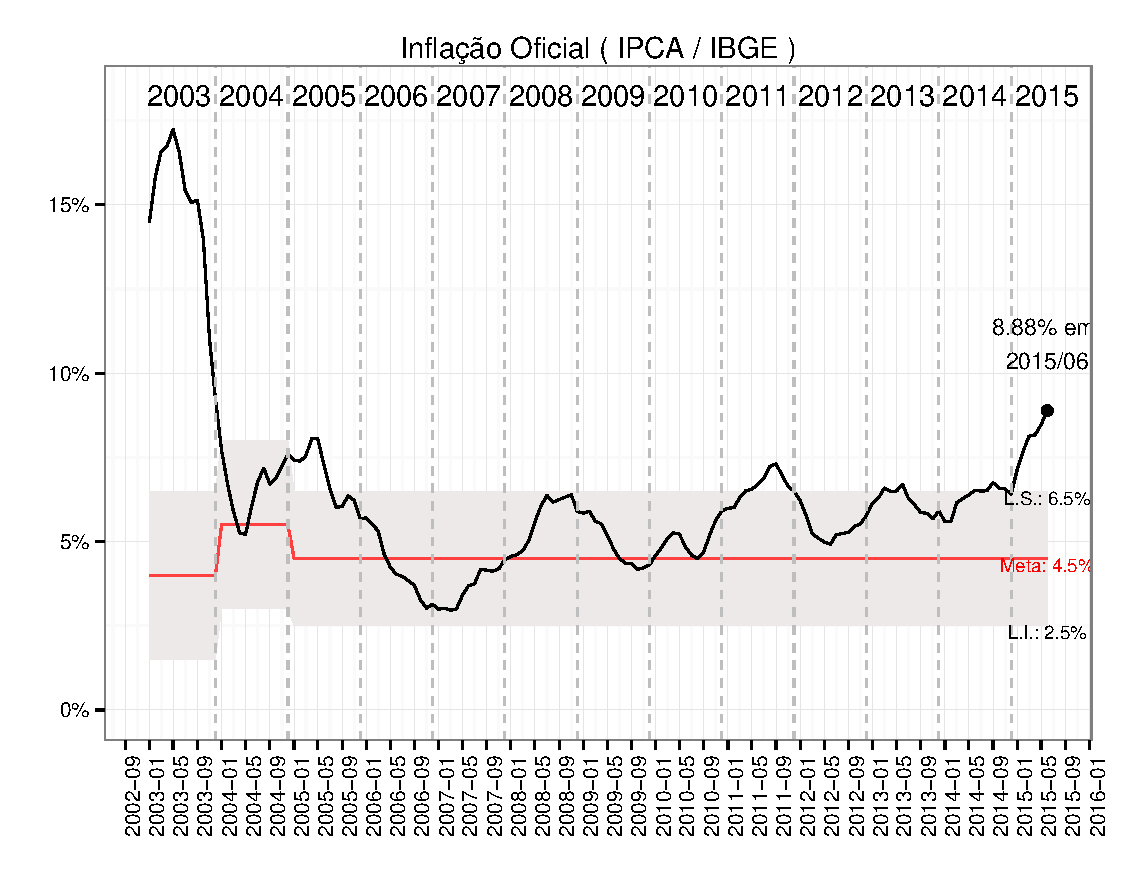
\includegraphics{Inflacao.pdf}
  \end{minipage}
\end{figure}


\textbf{Índice Nacional de Preços ao Consumidor Amplo}, também do IBGE, calculado desde 1980, semelhante ao INPC, porém refletindo o custo de vida para famílias com renda mensal de 1 a 40 salários mínimos.

A pesquisa é feita em nove regiões metropolitanas (São Paulo, Rio de Janeiro, Belo Horizonte, Porto Alegre, Recife, Belém, Fortaleza, Salvador e Curitiba) além dos municípios de Goiânia e Brasília, tendo sido escolhido como alvo das metas de inflação no Brasil

A partir do dia 30 de junho de 1999, o CMN (Conselho Monetário Nacional) estabeleceu o IPCA como índice oficial de inflação do Brasil.

\textbf{Fonte}: IBGE/Sistema Nacional de Índices de Preços ao Consumidor (IPCA e INPC)

\pagebreak

Abaixo há o detalhamento por grupo que constitui o índice IPCA.

\begin{figure}[!ht]
  \begin{minipage}{1.0\textwidth}
    \centering
      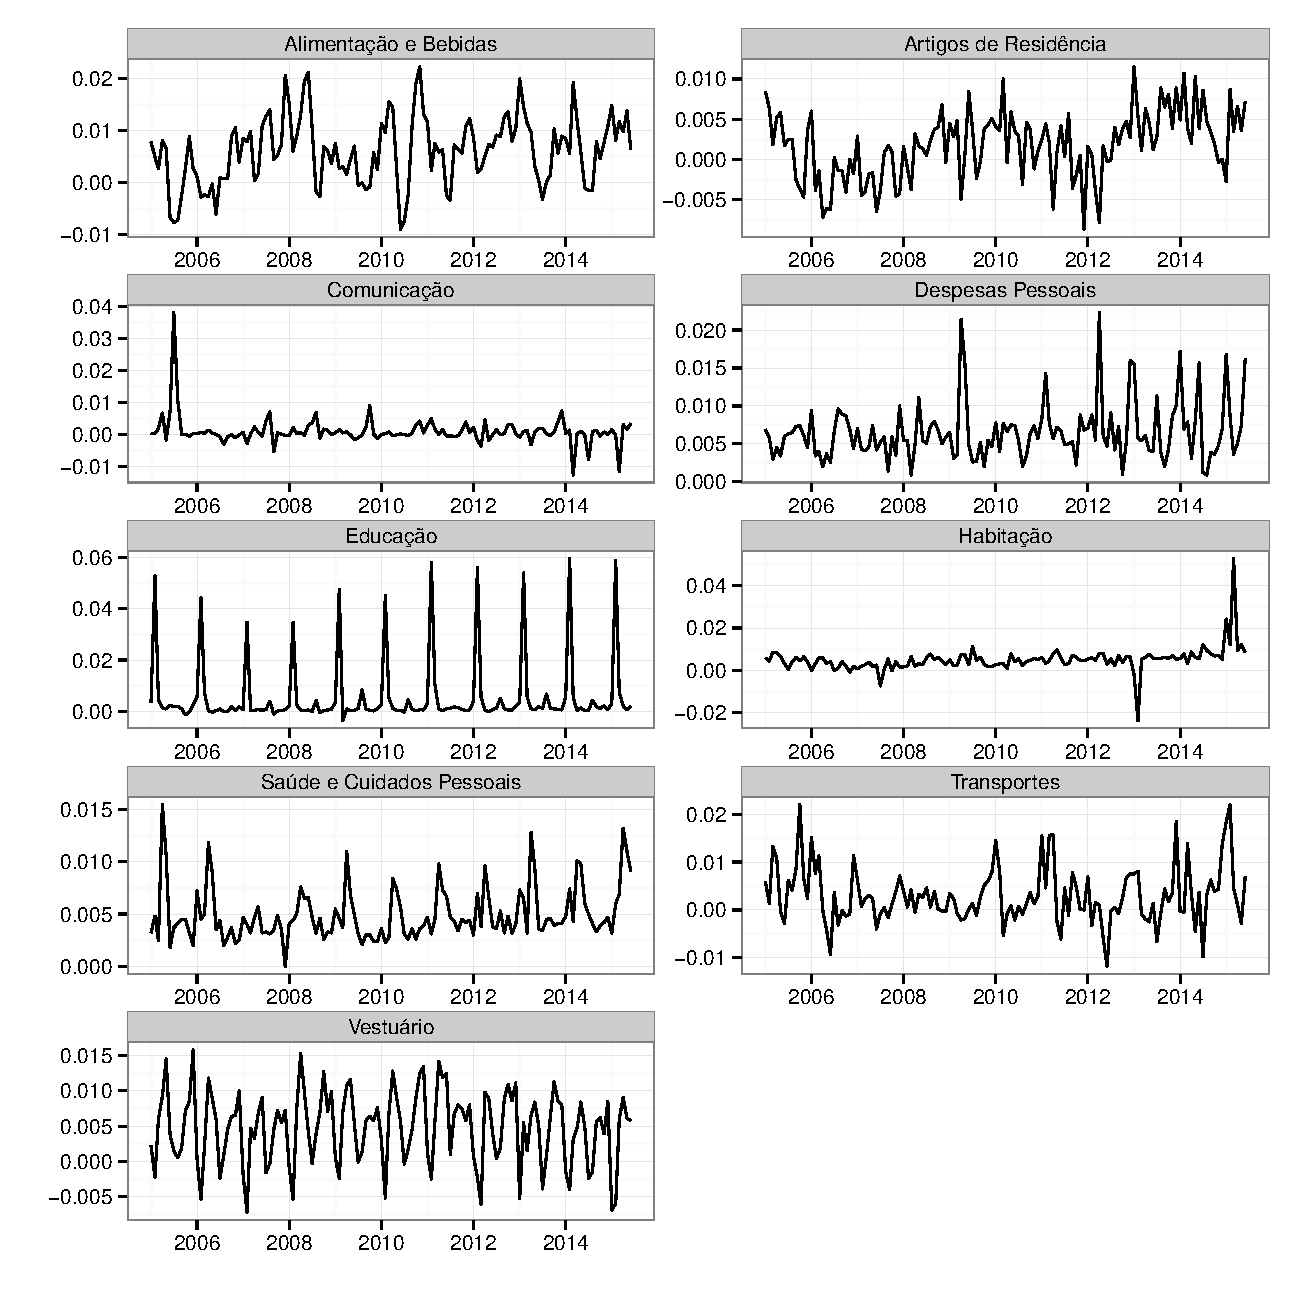
\includegraphics[width=\textwidth]{IPCAporGrupo.pdf}
  \end{minipage}
\end{figure}

\pagebreak

Mensalmente o Comite de Política Monetária (COPOM) divulga as metas de inflacao para os próximos anos. Abaixo encontra-se o documento mais recente disponível para consulta no site do Bacen.

\begin{figure}[!ht]
  \begin{minipage}{\textwidth}
    \centering
      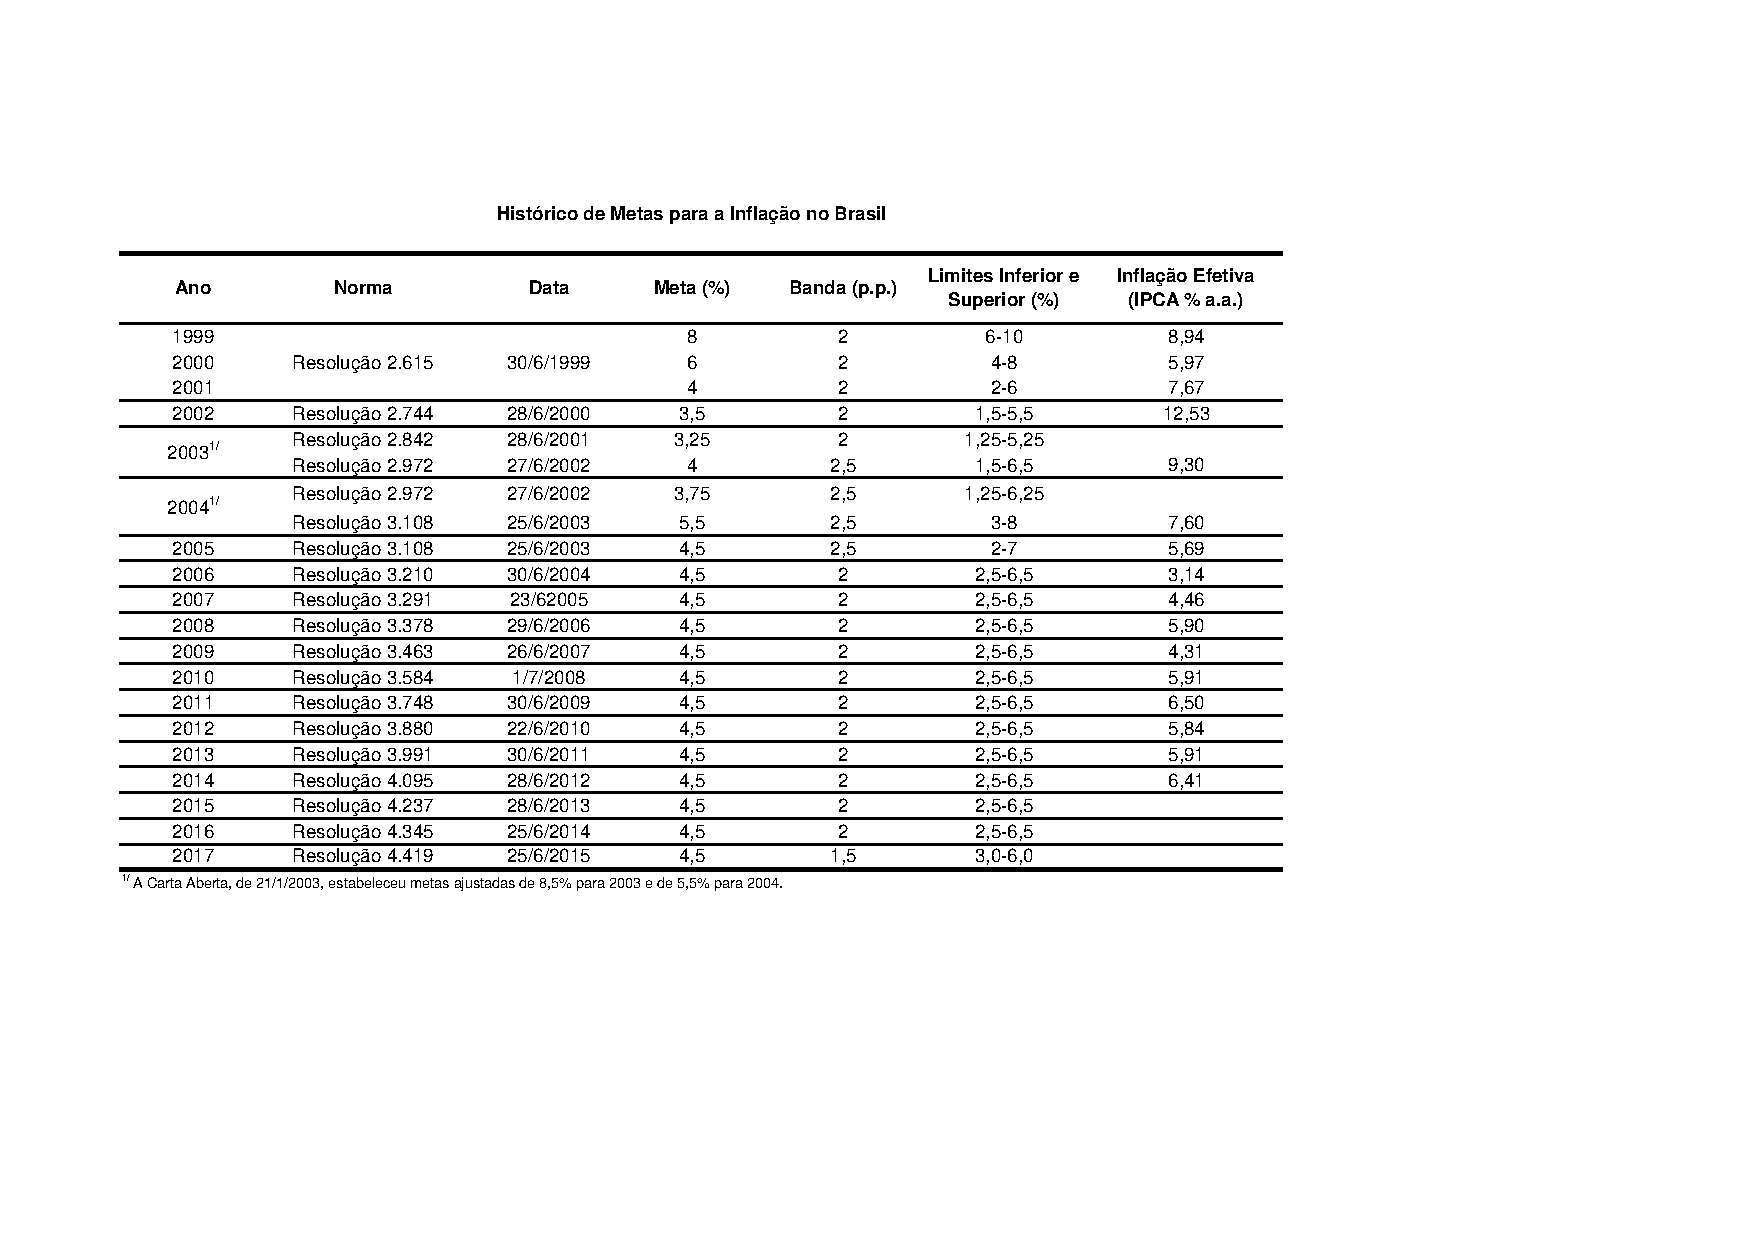
\includegraphics[width=1.4\textwidth]{BacenHistoricoMetas.pdf}
  \end{minipage}
\end{figure}

\pagebreak

Reproduzindo a excelente análise do Atirei o Pau no Gráfico...

\begin{figure}[!ht]
  \begin{minipage}{0.70\textwidth}
    \centering
      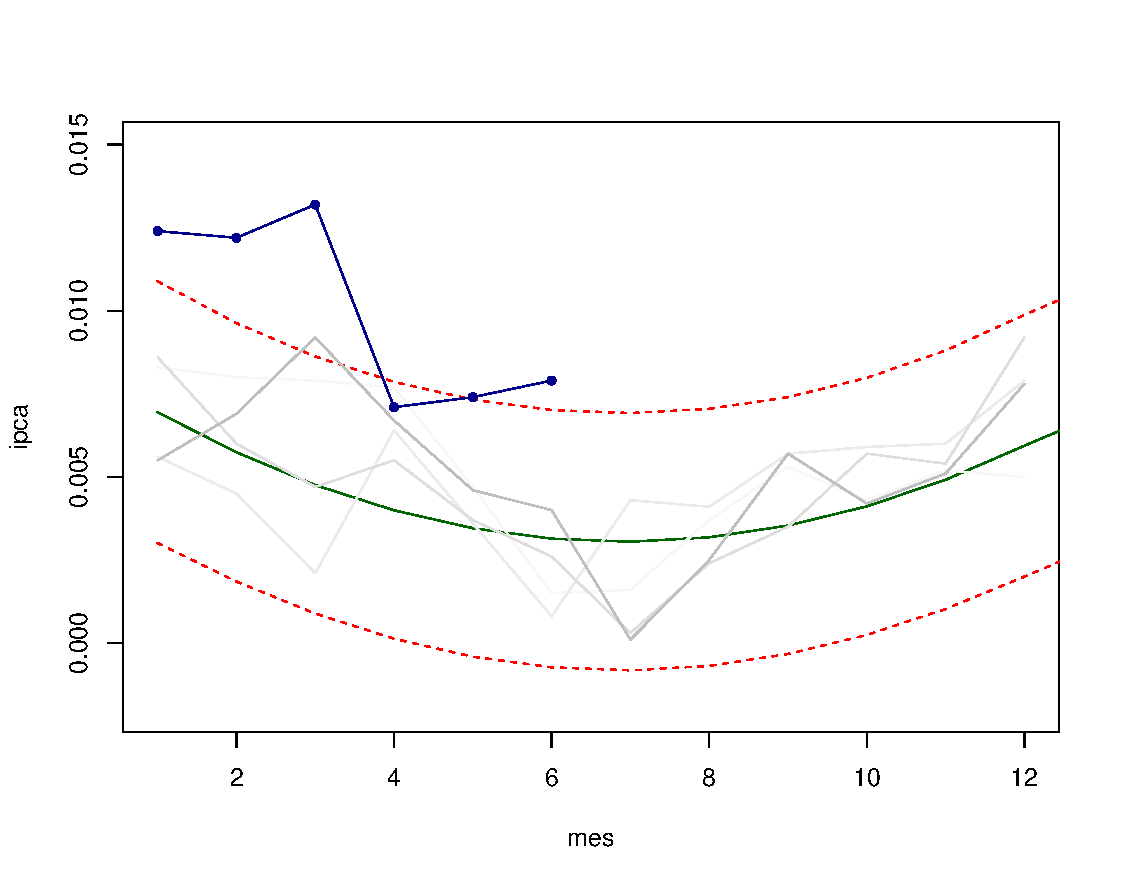
\includegraphics{IPCAatirei.pdf}
  \end{minipage}
\end{figure}

\pagebreak


\end{document}
